%%
%% Author: stefano
%% 3/30/19
%%

\documentclass[../../documentazione.tex]{subfiles}

\begin{document}

    \section{Macro richiesta}\label{sec:macro-richiesta}

    La macro richiesta per il progetto riguarda lo sviluppo di un software gestionale ERP per la gestione aziendale
    della produzione di Biciclette.
    Lo scopo finale degli sviluppatori é di rendere il software completamente personalizzabile e configurabile
    al fine di adattarlo alle molteplici necessitudini del mercato.

    Lo sviluppo sará quindi inizialmente rivolto alla creazione e messa in opera di un software gestionale MRP
    comprendente la maggior parte delle funzionalitá di ottimizzazione del processo, per poi evolverlo in un completo
    gestionale ERP.
    L'aggiornamento sará chiavi in mano e si porrá l'obbiettivo di mantenere attiva la linea di produzione
    durante i cambiamenti.

    \section{Obiettivi}\label{sec:obbiettivi}

    L'obbiettivo finale concordato consiste nella realizzazione del software.
    Il software dovrá consentire la gestione del magazzino, con la determinazione delle giacenze e la gestione delle commesse.
    Le commesse dovranno essere assegnate ai centri di lavoro configurati rispettandone il carico massimo e le tempistiche.
    Mediante la gestione delle commesse si avrá anche la gestione degli ordini, sia di produzione che di fornitura:
    sará dunque possibile ottimizzare gli ordini esterni grazie a un sistema di ottimizzazione delle date.

    Il software, essendo altamente configurabile, potrá essere rivenduto ad altre aziende dello stesso genere,
    garantendo un'automazione della catena di produzione e un'elevata flessibilitá di gestione del magazzino.

    Grazie a queste features vi é una possibilitá di guadagno distribuita negli anni.

    Una possibile metodologia di vendita potrebbe permettere un pagamento mensile della piattaforma, che potrebbe essere
    trasportata nel cloud in un futuro, oppure un pagamento sostanzioso immediato per la messa in opera locale.
    In tal caso, i costi di manutenzione non saranno compresi.

    \begin{figure}
        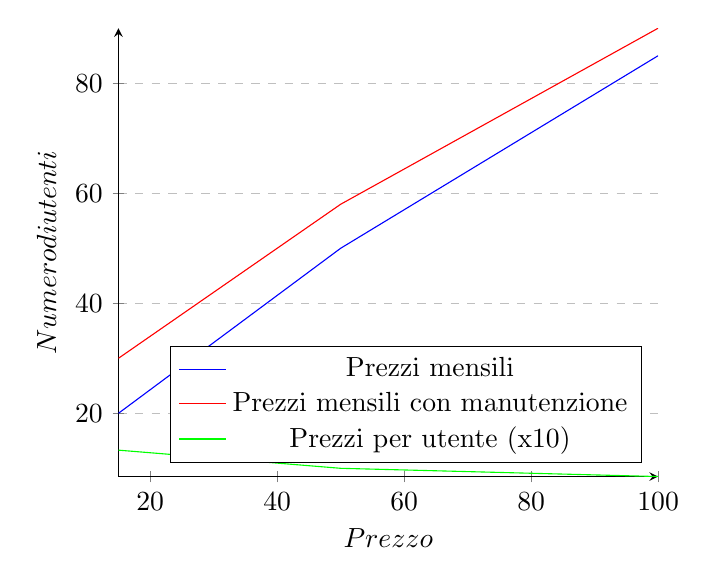
\begin{tikzpicture}
            \begin{axis}[
            axis lines = left,
            xlabel = $Prezzo$,
            ylabel = {$Numero di utenti$},
            legend pos=south east,
            ymajorgrids=true,
            grid style=dashed,
            ]
                \addplot[color = blue]
                coordinates {
                (15,20)(50,50)(100,85)
                };
                \addlegendentry{Prezzi mensili}

                \addplot[color = red]
                coordinates {
                (15,30)(50,58)(100,90)
                };
                \addlegendentry{Prezzi mensili con manutenzione}

                \addplot[color = green]
                coordinates {
                (15,13.3)(50,10)(100,8.5)
                };
                \addlegendentry{Prezzi per utente (x10)}
            \end{axis}
        \end{tikzpicture}
        \caption{Grafico dei prezzi per abbonamenti mensili}
    \end{figure}

    \begin{table}[H]
        \caption{Prezzi mensili della suite}
        \begin{tabular}{l|llll}
            \textbf{Numero di utenti} & \textbf{Prezzo Mensile} & \textbf{Prezzo+manutenzione} & \textbf{USD/utente} &  \\ \cline{1-4}
            15 & 20\$            & 30\$                         & 1.30\$ / 2\$          &  \\
            50 & 50\$            & 58\$                         & 1\$ / 1.16\$          &  \\
            100 & 85\$            & 90\$                         & 0.85\$ / 0.90\$       &  \\
            +100 & Contattaci & & &
        \end{tabular}
    \end{table}

    \begin{table}[H]
        \caption{Prezzi di acquisto}
        \begin{tabular}{ll}
            \textbf{Installazione locale} & \textbf{5400\$}\\
            Manutenzione & 600\$          \\
            Manutenzione base dati & 620\$          \\
        \end{tabular}
    \end{table}

    \section{Benefici}\label{sec:benefici}

    \subsection*{Benefici monetari}\label{subsec:benefici-monetari}
    La gestione degli ordini migliorata permette di ottimizzare le quantitá a magazzino e garantisce una gestione
    ottimizzata dei capitali.
    Una riorganizzazione del personale é ora possibile.

    \subsection*{Alta configurabilitá}\label{subsec:alta-configurabilitá}
    Le possibilitá di configurazione elevate permettono all'utente di adattare il software in tutti i suoi ambiti
    alla struttura aziendale.
    La libertá di scelta nelle configurazioni, seppur costringendo la configurazione a personale qualificato,
    permette un elevato numero di clienti.

    \subsection*{Gestione ottimizzata delle risorse}\label{subsec:gestione-ottimizzata-delle-risorse}
    La gestione del magazzino verrá ottimizzata nelle quantitá: la gestione della merce a commessa permetterá la limitazione
    delle quantitá nel tempo.
    La gestione degli ordini consentirá di ottimizzare le quantitá acquistate per usufruire delle leggi dell'economia di scala.

    \subsection*{Riduzione dei tempi}\label{subsec:riduzione-dei-tempi}
    Le tempistiche di produzione possono essere ottimizzate mantenendo stabile il carico di lavoro interno.
    Le tempistiche possono essere ulteriormente abbassate consentendo al software di stabilire le quantitá da produrre per
    mantenere il carico dei centri di lavoro costante.

    \section{SOAP - L'azienda del futuro}\label{sec:soap---l'azienda-del-futuro}
    SOAP è una società snella, nata a Brescia nel 1915 e in continua espansione.
    L'idea che guida l'attività è favorire lo sviluppo di un'impresa moderna, focalizzata sui talenti che possono fare
    la differenza per trovare le più opportune soluzioni ai problemi di gestione per ogni tipologia di azienda.

    Ciò che SOAP fornisce sono strumenti che permettono alle persone di lavorare nel modo più efficace,
    valorizzando le proprie competenze e ottimizzando il proprio tempo.

    L'obbiettivo è convertire l'idea dei sistemi informativi da male necessario a fattore competitivo e di semplificazione del business.

    La crescita maturata in questi anni è una combinazione di fattori umani e conoscenze tecniche di altissimo livello.
    I nostri consulenti stabiliscono un rapporto mirato a durare nel tempo: a chi decide di rivolgersi a SOAP è dedicato
    un approccio che supera il rapporto fornitore-cliente, puntando a una reciproca crescita per il raggiungimento degli obbiettivi stabiliti.

    La nostra consulenza verte sulla concretezza, la competenza, l'impegno e la passione:
    punti di forza molto apprezzati da chi ci ha affidato la gestione dei propri sistemi e che creano le migliori condizioni
    per ridurre il time-to-market.

    Un'impresa di qualunque dimensione oggi non può permettersi di sfuggire alle trasformazioni tecnologiche in corso che,
    se ben sfruttate, permettono una gestione serena ed efficace del business.
    Ogni organizzazione ha a che fare con ingenti quantità d'informazioni che devono essere facilmente catalogate,
    analizzate e messe in circolazione all'interno dei dipartimenti aziendali.
    I sistemi informativi devono essere vissuti come un reale fattore competitivo e di successo dell'impresa:
    noi possiamo aiutarti a ottimizzare i processi di lavoro.

    Il nostro impegno è mutuare i migliori progetti internazionali, punti di riferimento dei più innovativi modelli di organizzazione,
    nell'ambito concreto in cui opera ogni azienda. Occorre capire le specifiche esigenze del cliente:
    le logiche di una piccola realtà lavorativa sono diverse da quelle della grande impresa.

    \subsection{Struttura aziendale}\label{subsec:struttura-aziendale}
    La struttura aziendale é una struttura organizzata gerarchicamente dove, per mancanza di personale, i componenti sono
    costretti a sopperire determinate mansioni.

    \begin{figure}
        \begin{tikzpicture}
            \umlclass[x=3]{Project Management}{Stefano Fontana \\ Ramy Abdulkadir}{}
            \umlclass[x=0, y=-5]{Backend}{Stefano Fontana \\ Luca Vezzoli}{}
            \umlclass[x=0, y=-9]{Testing}{Torli Francesco}{}
            \umlclass[x=3.5, y=-5]{Frontend}{Ramy Abdulkadir \\ Sciola Lorenzo}{}
            \umlclass[x=3.5, y=-9]{Testing -}{Frusca Lorenzo}{}
            \umlclass[x=7.2, y=-5]{Relazioni esterne}{Pacecchi Paolo}{}

            \umlHVassoc[]{Project Management}{Backend}
            \umlHVassoc[]{Project Management}{Frontend}
            \umlHVassoc[]{Project Management}{Relazioni esterne}
            \umlHVassoc[]{Backend}{Testing}
            \umlHVassoc[]{Frontend}{Testing -}
        \end{tikzpicture}
        \caption{Organigramma}
    \end{figure}

    L'azienda si comporrá di tre unitá organizzative di cui due dedicate allo sviluppo informatico, mentre la restante
    si occuperá della gestione dei rapporti con stakeholders e con esterni, divenendo tramite e filtro per gli sviluppatori.
    Le U.O. dedicate agli sviluppi backend e frontend avranno come subordinate le relative U.O. di testing,
    al fine di garantire un codice sempre funzionante e mantenibile.
    La direzione del progetto é condivisa invece tra due sviluppatori provenienti da due U.O. diverse, in modo tale
    da mantenere una situazione di paritá e permettere che le decisioni siano fattibili per ambo le parti.
    Inoltre, la vicinanza dei due membri permetterá una comunicazione fluida tra le U.O.

    \subsection{Stakeholders}\label{sec:steackholders}
    La realtá aziendale di una piccola azienda come SOAP puó contare su grandi nomi internazionali come
    \textit{Elon Musk}, \textit{Linus Torvalds} e \textit{Michelito Carnevalovskij}.
    Hacker rinomati come \textit{codingdecoding} supportano la teconologia con consigli relativi alla sicurezza.

    \section{Analisi dei requisiti}\label{sec:analisi-dei-requisiti}

    \begin{figure}
        \begin{tikzpicture}
            \begin{umlsystem}[x=4, fill=red!10]{Cibicletta-industries}

                \umlusecase[y=0, x=0]{Nuova Commessa}
                \umlusecase[y=0, x=4.5]{Gestione commesse}

                \umlusecase[y=-2, fill=blue!20]{Gestione Magazzino}

                \umlusecase[y=-4, x=0, fill=green!20]{Nuovo Ordine}
                \umlusecase[y=-4, x=4, fill=green!20]{Gestione ordini}
                \umlusecase[y=-6, x=0, fill=green!20]{Ottimizza Ordini}

                \umlusecase[y=-8, x=0, fill=red!20]{Gestione reparti}
                \umlusecase[y=-8, x=4, fill=red!20]{Scheduler}

            \end{umlsystem}

        \end{tikzpicture}
        \caption{Diagramma di caso d'uso per l'analisi dei requisiti}
    \end{figure}

    \begin{sidewaysfigure}[ht]
        \resizebox{!}{.6\linewidth}{
        \begin{tikzpicture}
            \begin{umlseqdiag}
                \umlactor[x=0, class=C]{Cliente}
                \umlactor[x=5, class=C]{RProg}
                \umlobject[x=10, no ddots]{Reparto X}
                \umlactor[x=15, class=C]{Fornitore}
                \umlactor[x=20, class=C]{Operaio}
                \umlmulti[x=25, class=G]{Magazzino}

                \begin{umlcall}[op=Ordine]{Cliente}{RProg}
                    \begin{umlcall}[op=Ordine]{RProg}{Fornitore}
                        \begin{umlcall}[op=Consegna, type=return]{Fornitore}{Magazzino}
                        \end{umlcall}
                    \end{umlcall}

                    \begin{umlcall}[op=Crea Task]{RProg}{Reparto X}
                        \begin{umlfragment}[type=alt, label=Ctrl OK, inner xsep=9]
                            \begin{umlcall}[op=Incarica, return=Pezzo]{Reparto X}{Operaio}
                                \begin{umlcall}[op=Richiede, return=Materiale]{Operaio}{Magazzino}
                                \end{umlcall}
                                \begin{umlcallself}[op=Crea]{Operaio}
                                \end{umlcallself}
                            \end{umlcall}
                            \begin{umlcallself}[op=Controllo]{Reparto X}
                            \end{umlcallself}

                            \umlfpart[]

                            \begin{umlcall}[op=Deposita]{Reparto X}{Magazzino}
                            \end{umlcall}
                        \end{umlfragment}

                        \begin{umlcall}[op=Incarica Assemblaggio, return=Pezzo]{Reparto X}{Operaio}
                            \begin{umlcallself}[op=Assembla]{Operaio}
                            \end{umlcallself}
                        \end{umlcall}

                        \begin{umlcall}[op=Consegna, type=return]{Reparto X}{Cliente}
                        \end{umlcall}
                    \end{umlcall}

                \end{umlcall}

            \end{umlseqdiag}
        \end{tikzpicture}
        }
        \caption{Diagramma di sequenza ordine}
    \end{sidewaysfigure}

    \clearpage
    \section{WBS}\label{sec:wbs}
    La WBS per il sistema (vedi Fig. 1.5) divide l'intero applicativo in due sezioni:
    una sezione Backend che manterrá l'autenticazione degli utenti e gestirá il database,
    e una sezione Frontend per l'interazione con l'utente.


    \begin{figure}
        \resizebox{.63\linewidth}{!}{
        \begin{tikzpicture}
            \umlclass[x=4]{1}{Software Applicativo}{}
            \umlclass[x=0, y=-2]{11}{Backend}{}
            \umlclass[x=1.5, y=-4]{111}{Database}{}
            \umlclass[x=1.5, y=-6]{112}{Web Service}{}
            \umlclass[x=3, y=-8]{1121}{REST}{}
            \umlclass[x=3, y=-10]{1122}{Auth}{}
            \umlclass[x=1.5, y=-12]{113}{Motore}{}
            \umlclass[x=3, y=-14]{1131}{Carichi}{}
            \umlclass[x=3, y=-16]{1132}{Fabbisogni}{}
            \umlclass[x=3, y=-18]{1133}{Date}{}
            \umlclass[x=1.5, y=-20]{114}{Motore PDF}{}

            \umlclass[x=8, y=-2]{12}{Frontend}{}
            \umlclass[x=9.5, y=-4]{121}{Login}{}
            \umlclass[x=9.5, y=-6]{122}{Dashboard}{}
            \umlclass[x=9.5, y=-8]{123}{Funzioni}{}
            \umlclass[x=12, y=-10]{1231}{Amministrazione}{}
            \umlclass[x=12, y=-12]{1232}{Configs}{}
            \umlclass[x=12, y=-14]{1233}{Gest. Ordini}{}
            \umlclass[x=12, y=-16]{1234}{Gest. Commesse}{}
            \umlclass[x=12, y=-18]{1235}{Gest. Magazzino}{}

            \umlHVassoc[]{1}{11}
            \umlHVassoc[]{1}{12}

            \umlVHassoc[]{11}{111}
            \umlVHassoc[]{11}{112}
            \umlVHassoc[]{11}{113}
            \umlVHassoc[]{11}{114}
            \umlVHassoc[]{112}{1121}
            \umlVHassoc[]{112}{1122}
            \umlVHassoc[]{113}{1131}
            \umlVHassoc[]{113}{1132}
            \umlVHassoc[]{113}{1133}

            \umlVHassoc[]{12}{121}
            \umlVHassoc[]{12}{122}
            \umlVHassoc[]{12}{123}
            \umlVHassoc[]{123}{1231}
            \umlVHassoc[]{123}{1232}
            \umlVHassoc[]{123}{1233}
            \umlVHassoc[]{123}{1234}
            \umlVHassoc[]{123}{1235}

        \end{tikzpicture}
        }
        \caption{Work breakdown structure}
    \end{figure}

    \clearpage

    \begin{ganttchart}[
    canvas/.append style={fill=none, draw=black!5, line width=.75pt},
    hgrid style/.style={draw=black!5, line width=.75pt},
    vgrid={*1{draw=black!5, line width=.75pt}},
    title/.style={draw=none, fill=none},
    title label font=\bfseries\footnotesize,
    title label node/.append style={below=7pt},
    include title in canvas=false,
    bar label font=\mdseries\small\color{black!70},
    bar label node/.append style={left=2cm},
    bar/.append style={draw=none, fill=black!63},
    bar incomplete/.append style={fill=barblue},
    bar progress label font=\mdseries\footnotesize\color{black!70},
    group incomplete/.append style={fill=groupblue},
    group left shift=0,
    group right shift=0,
    group height=.5,
    group peaks tip position=0,
    group label node/.append style={left=.6cm},
    group progress label font=\bfseries\small
    link label font=\scriptsize\bfseries,
    link label node/.append style={below left=-2pt and 0pt}
    ]{1}{21}
        \gantttitle{2019}{21} \\
        \gantttitlelist{1,...,21}{1} \\

        \ganttbar{Web Service}{1}{2}\\
        \ganttbar{Database}{1}{3}\\

        \ganttbar{Autenticazione}{4}{6}
        \ganttlink[link type=dr]{elem0}{elem2}
        \ganttlink[link type=dr]{elem1}{elem2}\\

        \ganttbar{REST}{7}{11}
        \ganttlink[link type=dr]{elem2}{elem3}\\

        \ganttbar{MOCK}{4}{5}
        \ganttlink[link type=dr]{elem1}{elem4}\\

        \ganttbar{Libreria grafica}{1}{3}\\
        \ganttbar{Libreria PDF}{1}{4}\\

        \ganttbar{Magazzino}{6}{11}
        \ganttlink[link type=dr]{elem4}{elem7}\\
        \ganttbar{Login}{6}{11}
        \ganttlink[link type=dr]{elem4}{elem8}\\

        \ganttbar{Amministrazione}{6}{11}
        \ganttlink[link type=dr]{elem4}{elem9}
        \ganttlink[link type=dr]{elem5}{elem9}
        \ganttlink[link type=dr]{elem6}{elem9}\\
        \ganttbar{Commesse}{6}{11}
        \ganttlink[link type=dr]{elem4}{elem10}
        \ganttlink[link type=dr]{elem5}{elem10}
        \ganttlink[link type=dr]{elem6}{elem10}\\
        \ganttbar{Ordini}{6}{11}
        \ganttlink[link type=dr]{elem4}{elem11}
        \ganttlink[link type=dr]{elem5}{elem11}
        \ganttlink[link type=dr]{elem6}{elem11}\\

        \ganttbar{Configs}{12}{16}
        \ganttlink[link type=dr]{elem7}{elem12}
        \ganttlink[link type=dr]{elem8}{elem12}
        \ganttlink[link type=dr]{elem9}{elem12}
        \ganttlink[link type=dr]{elem10}{elem12}
        \ganttlink[link type=dr]{elem11}{elem12}\\

        \ganttbar{Dashboard}{17}{21}
        \ganttlink[link type=dr]{elem12}{elem13}\\

    \end{ganttchart}

    \section{Gantt chart}\label{sec:gantt-chart}
    L'elenco delle attivitá di sviluppo e delle precedenze viene descritto nel diagramma di Gantt.
    Le deliverable consistono in tutti quei macro componenti che compongono il sistema:\\
    - Infrastruttura di test\\
    - Backend\\
    - Frontend\\
    - Consegna

    \begin{table}[]
        \begin{tabular}{lllll}
            \hline
            \multicolumn{1}{|l}{\textbf{Milestone}} & \textbf{Componente}                   & \textbf{Start} & \textbf{Durata} & \multicolumn{1}{l|}{\textbf{Assegnato}} \\ \hline
            \textit{\textbf{Backend}}               & \multicolumn{1}{l|}{\textbf{}}        & \textbf{}                & \textbf{}       &                                         \\ \hline
            & \multicolumn{1}{l|}{Web Service}      & 0                        & 2               & Abdulkadir                              \\
            CRIT& \multicolumn{1}{l|}{Database}         & 0                        & 3               & Vezzoli                                 \\
            & \multicolumn{1}{l|}{Autenticazione}   & 4                        & 3               & Fontana                                 \\
            & \multicolumn{1}{l|}{REST}             & 7                        & 5               & Vezzoli                                 \\
            \textit{\textbf{TI}}   & \multicolumn{1}{l|}{}                 &                          &                 &                                         \\ \hline
            CRIT& \multicolumn{1}{l|}{MOCK}             & 4                        & 2               & Fontana                                 \\
            \textit{\textbf{Frontend}}              & \multicolumn{1}{l|}{}                 &                          &                 &                                         \\ \hline
            & \multicolumn{1}{l|}{Libreria grafica} & 0                        & 3               & Vezzoli                                 \\
            & \multicolumn{1}{l|}{Libreria PDF}     & 0                        & 5               & Fontana                                 \\
            CRIT& \multicolumn{1}{l|}{Magazzino}        & 6                        & 5               & Abdulkadir                              \\
            CRIT& \multicolumn{1}{l|}{Login}            & 6                        & 5               & Abdulkadir                              \\
            CRIT& \multicolumn{1}{l|}{Amministrazione}  & 6                        & 5               & Sciola                                  \\
            CRIT& \multicolumn{1}{l|}{Commesse}         & 6                        & 5               & Sciola                                  \\
            CRIT& \multicolumn{1}{l|}{Ordini}           & 6                        & 5               & Abdulkadir                              \\
            CRIT& \multicolumn{1}{l|}{Configs}          & 11                       & 5               & Frontend team                           \\
           CRIT & \multicolumn{1}{l|}{Dashboard}        & 16                       & 5               & Frontend team                           \\
            &                                       &                          &                 &                                         \\
            Sono omessi i test.                     &                                       &                          &                 &
        \end{tabular}
        \caption{Tabella distribuzione attivitá}
    \end{table}

    \section{Analisi dei rischi}\label{sec:analisi-dei-rischi}
    I rischi sono prettamente legati alle tempistiche, e il maggior rischio é rappresentato da ritardi nelle attivitá critiche.
    In particolare, nello sviluppo delle deliverable, sará necessario comprendere a fondo le richieste del cliente.


\end{document}
